\chapter{Persistence}

The persistence of our application is divided into persistent data and dynamic data. The persistent data is not modified by the user and can only be read which makes it easy to be later updated and fetched from a server. The dynamic data is frequently modified by the user and contains more user related information, such as his progress or his current total score.

\section{Persistent data}

The persistent data is stored as a JSON file inside the assets folder of our application. We decided to use JSON as data format because it's nowadays very popular, easy to read and has a short notation which minimizes the file size for transmission and storage. The JSON file is read at the launch of the application and parsed in order to create the objects needed for our application. In Figure~\ref{fig:JSONStructure} we can see the structure of our JSON file. It's a tree structure where the array cities is the root and contains several city objects. Each city object contains city related properties but also an array mysteries which contains several mystery objects. Finally, each mystery object contains mystery related properties but also an array challenges which contains several challenge objects.

\begin{figure}[H]
	\centering
	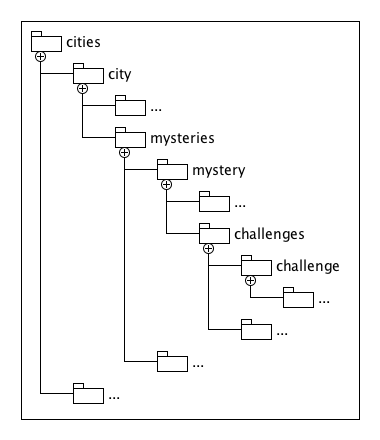
\includegraphics[scale=0.4]{Figures/JSONStructure}
	\caption{Diagram showing the structure of the persistent\_data.json file.}
	\label{fig:JSONStructure}
\end{figure}

\noindent
\\
Figure~\ref{fig:UMLDiagram} shows the UML diagram of the different classes and relationships concerning the persistent data. The class Home contains 0 or more cities. The class City contains 0 or more mysteries. The class Mystery contains 0 or more challenges. The class Challenge is an abstract class where the classes QuestionChallenge and CompassChallenge inherit from. Finally, ChallengeType, ChallengeState and MysteryState are enumeration types used across our application.

\begin{figure}[H]
	\centering
	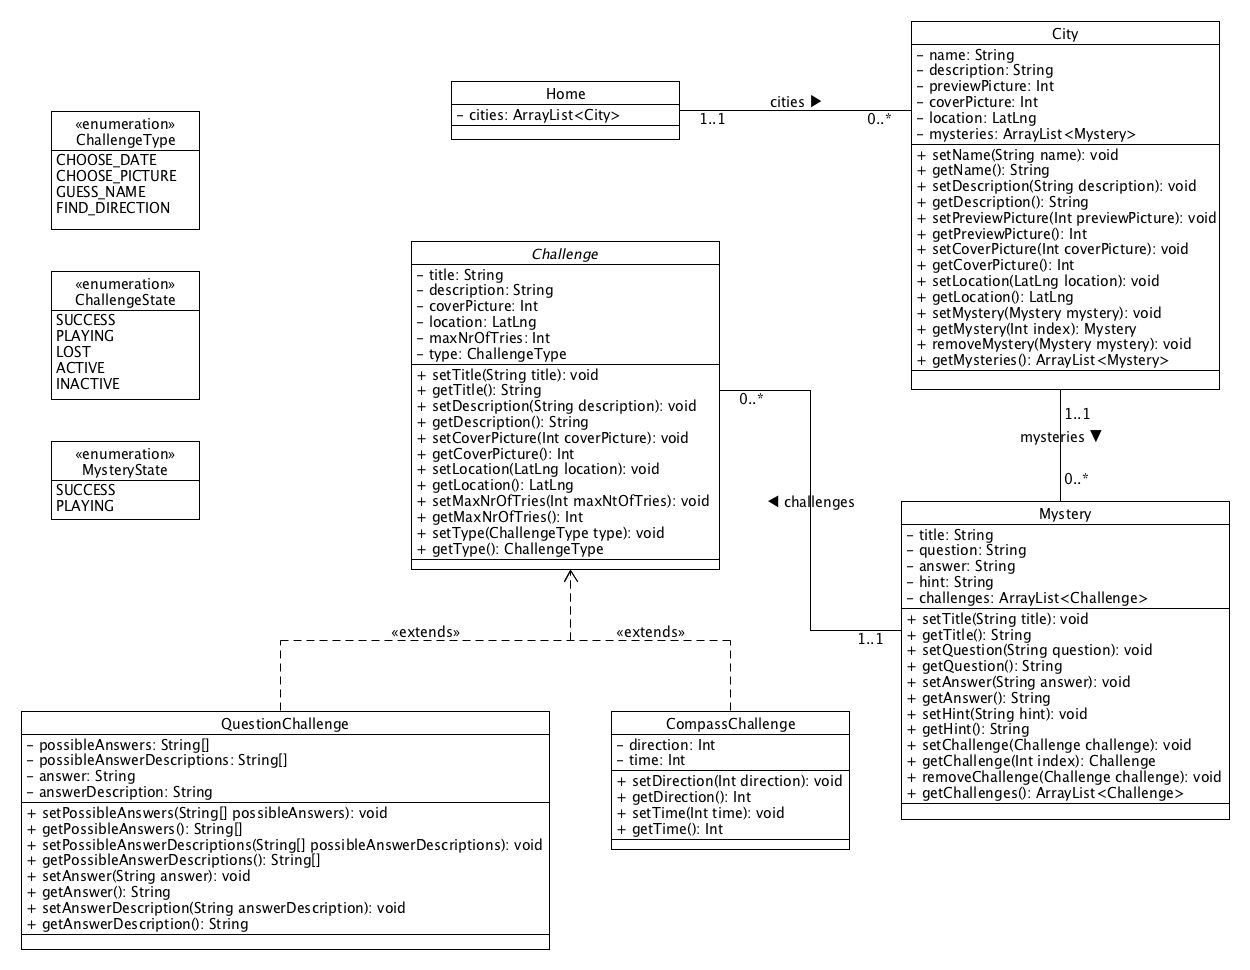
\includegraphics[scale=0.4]{Figures/PersistentData}
	\caption{UML diagram showing the different class and relationships concerning the persistent data.}
	\label{fig:UMLDiagram}
\end{figure}

\section{Dynamic data}

The dynamic data is stored as shared preferences. Shared preferences provide an easy interface to retrieve and modify primitive type values. Android saves shared preferences internally as files and takes care of their management. They are the perfect choice for storing settings and user related information. Our application uses the following shared preferences:

\begin{itemize}
	\item GELLE\_FRA\_PREFERENCES
	\item CATHEDRAL\_PREFERENCES
	\item PALAIS\_PREFERENCES
	\item PLACE\_GUILLAUME\_PREFERENCES
	\item PLACE\_CLAIREFONTAINE\_PREFERENCES
	\item MYSTERY\_1\_PREFERENCES
	\item SCORE\_PREFERENCES
\end{itemize}

\noindent
We store as shared preferences the progress of each challenge and mystery, but also the number of tries of each challenge and mystery. Depending on the challenge, we also store specific information about the current state of already selected buttons, pictures or words entered. The current total score of the user is also stored as a shared preference. The 'Settings' activity allows a user to delete all shared preferences and reset the state of the application.
